\begin{figure*}[t]
    \centering
    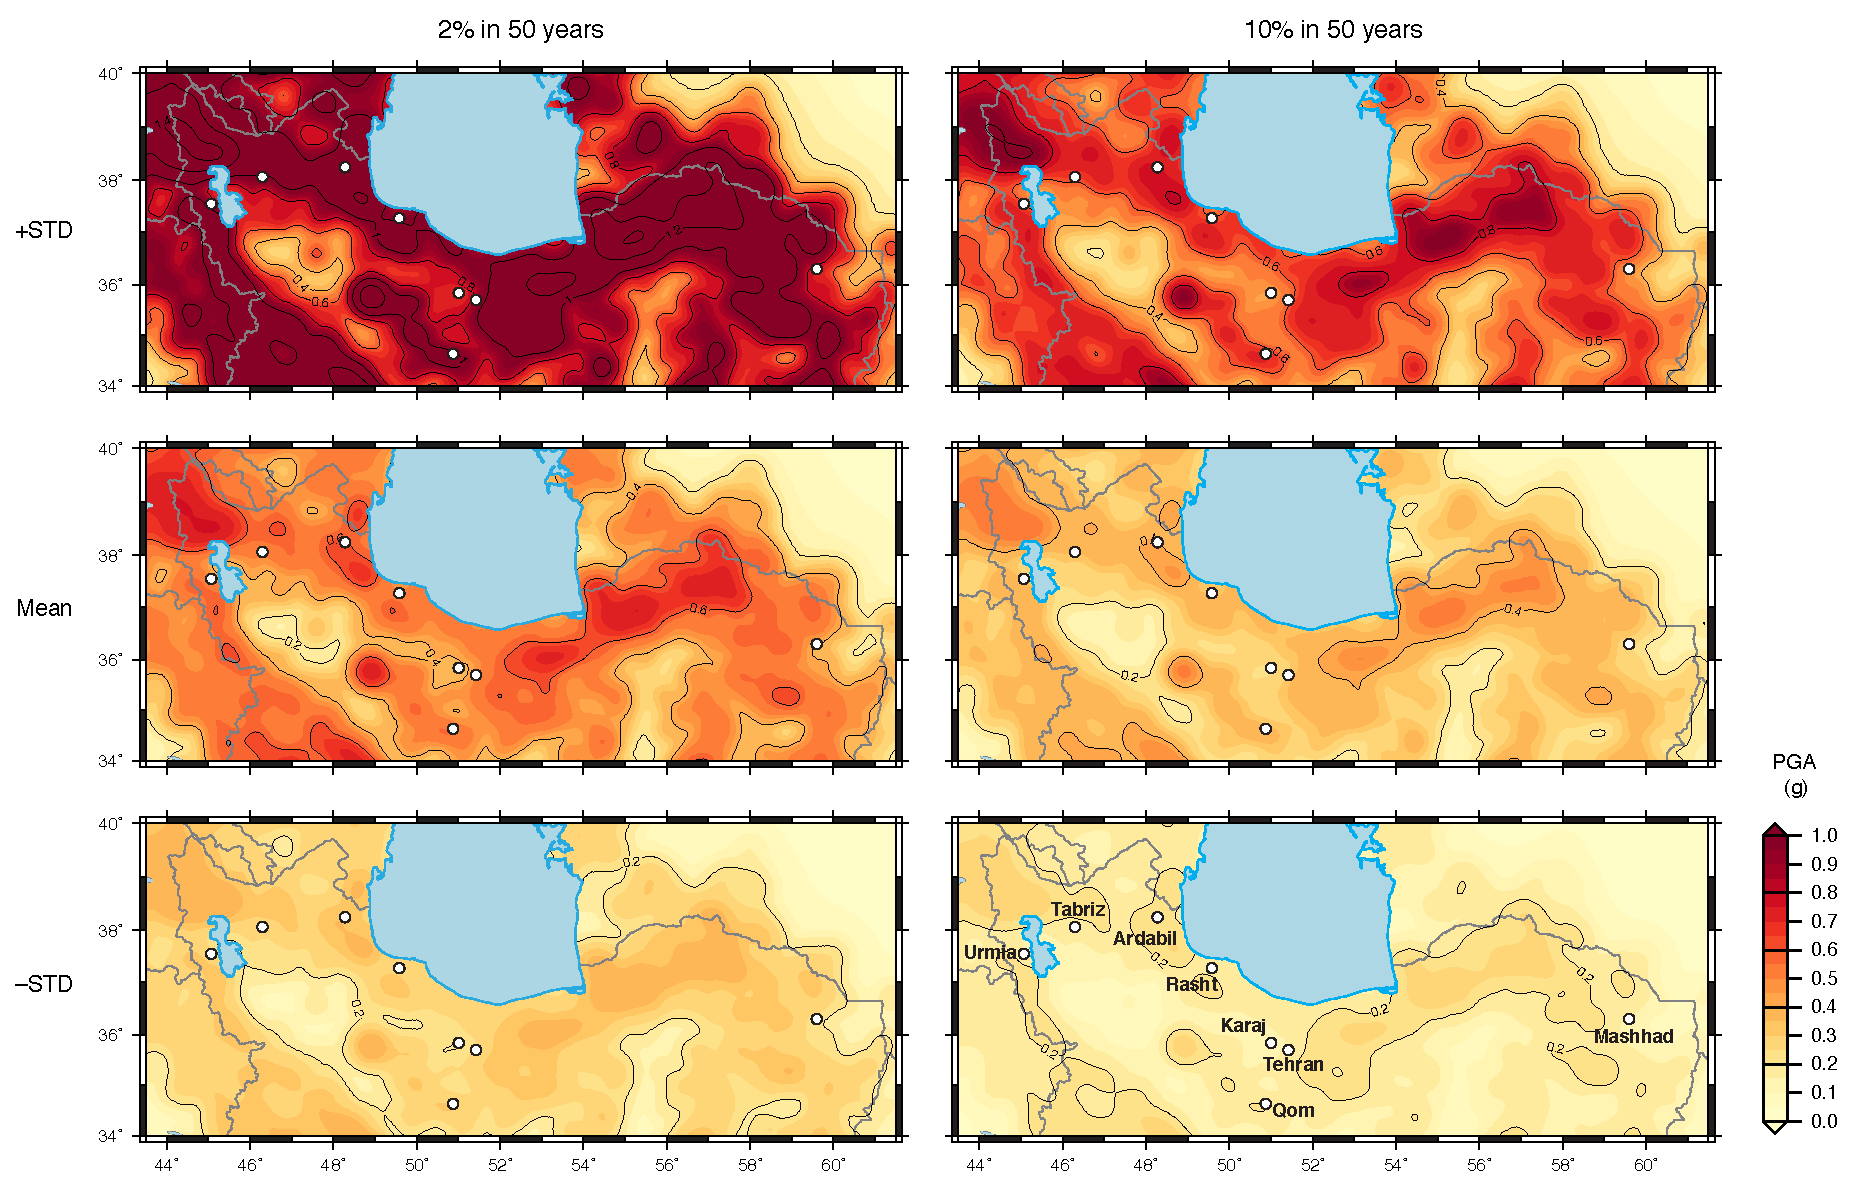
\includegraphics[width=\textwidth]{figures/pdf/figure-10.pdf}
    \caption{Expected mean peak ground acceleration (PGA) for 2 and 10 percent of probability of exceedance in 50 years for (a) the five-seismic regions R model and (b) the uniform seismic region U model.}
    \label{fig:pga}
\end{figure*}

\begin{figure*}[t]
    \centering
    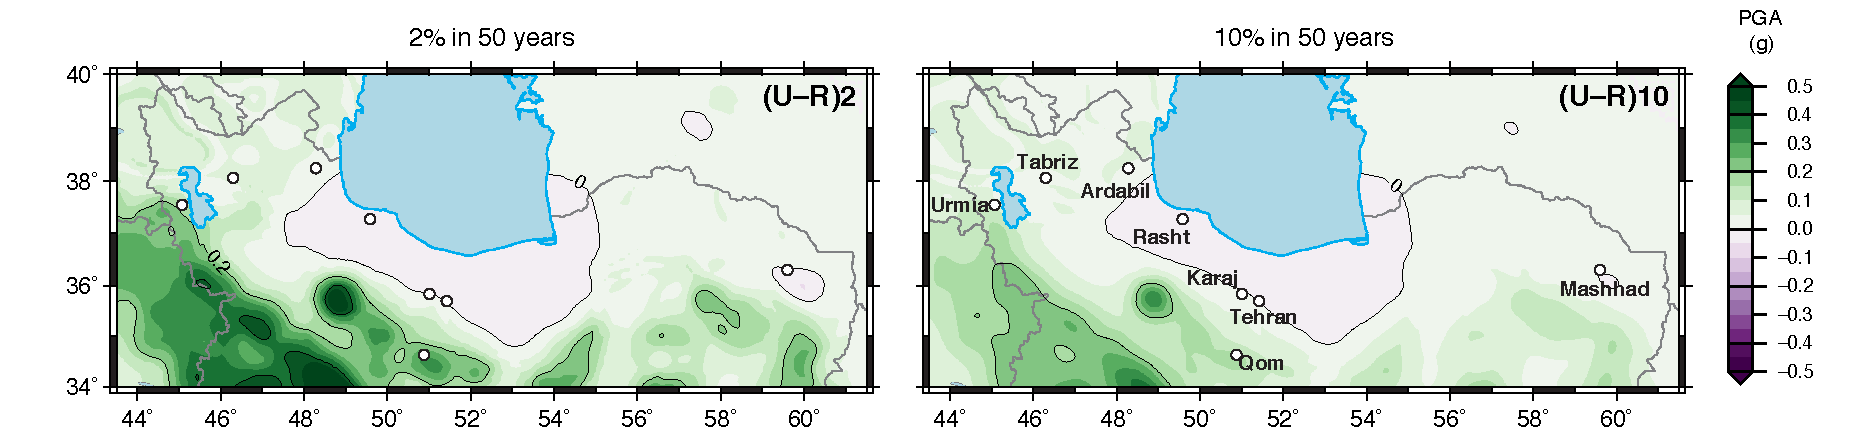
\includegraphics[width=\textwidth]{figures/pdf/figure-11.pdf}
    \caption{Difference between the mean PGA values from models U and R for 2 (left) and 10 (right) percent probabilities of exceedance in 50 years.}
    \label{fig:pga.diff}
\end{figure*}

\begin{figure*}[t]
    \centering
    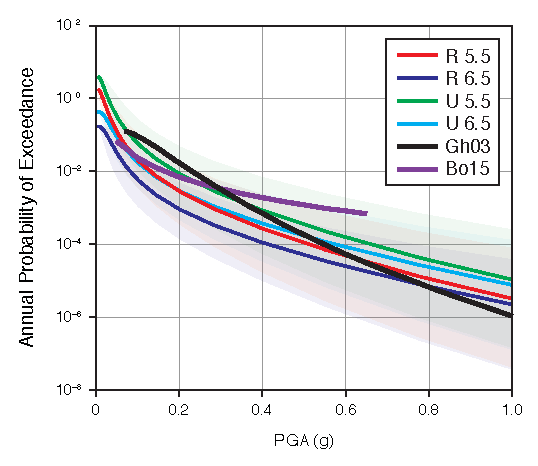
\includegraphics[width=\textwidth]{figures/pdf/figure-12.pdf}
    \caption{Expected PGA values throughout the region of interest for 2 (left) and 10 (right) percent probability of exceeding an earthquake magnitude $M_w$ 5 using the combined model (R,U) hazard calculations. Mean expected values are shown in the middle, whereas the top and bottom frames correspond to the results obtained using plus and minus one standard deviation.}
    \label{fig:pga.ru.std}
\end{figure*}


% \begin{table*}[t]
% \centering
% \caption{Comparison of expected PGA values for selected cities in northern Iran between results obtained in this study and those of others. For reference, the following codes are used. Va11: \citet{Vafaie2011}, Gh08: \citet{Ghodrati2008}, Bo15: \citet{Boostan2015}, Gh03: \citet{Ghodrati2003}, Ab14: \citet{Abdollahzadeh2014a}, Ra12: \citet{Rahgozar2012}, Ad13 \citet{Abdi2013}.}
% \begin{tabular}{lcccccccccccccccccccccc}
%     \hline
%     Cities  & Lon. & Lat. & R55  &      & R65  &      & U55  &      & U65  &      & RU55 &      & RU65 &      & RU5565 &    & 2800 & Zare 2012  & Golara2014 & Other References &      &      \\    
%             &      &      & 10\% &  2\% & 10\% &  2\% & 10\% &  2\% & 10\% &  2\% & 10\% &  2\% & 10\% &  2\% & 10\% &  2\% &      &            &            & 10\%       & 2\%        & Ref. \\
%     \hline
%     Urmia   & 45.1 & 37.6 & 0.28 & 0.45 & 0.19 & 0.34 & 0.28 & 0.47 & 0.21 & 0.37 & 0.28 & 0.46 & 0.20 & 0.36 & 0.26 & 0.40 & 0.30 & 0.35--0.50 & 0.3--0.5   &            &            &      \\
%     Tabriz  & 46.3 & 38.1 & 0.20 & 0.34 & 0.12 & 0.23 & 0.39 & 0.59 & 0.29 & 0.51 & 0.34 & 0.53 & 0.24 & 0.41 & 0.30 & 0.49 & 0.35 & 0.35--0.50 & 0.9--1.2   & 0.20--0.65 & 0.30--0.90 & Va11 \\
%     Ardabil & 48.3 & 38.3 & 0.23 & 0.38 & 0.14 & 0.27 & 0.47 & 0.70 & 0.37 & 0.57 & 0.39 & 0.58 & 0.28 & 0.50 & 0.36 & 0.55 & 0.30 & 0.35--0.50 & 0.5--0.7   &            &            &      \\
%     Rasht   & 49.6 & 37.3 & 0.25 & 0.39 & 0.16 & 0.29 & 0.36 & 0.54 & 0.26 & 0.45 & 0.31 & 0.50 & 0.22 & 0.38 & 0.28 & 0.46 & 0.30 & 0.50--0.65 & 0.5--0.7   & 0.10       & 0.20       & Gh08 \\
%             &      &      &      &      &      &             &      &      &      &      &      &      &      &      &      &      &            &            & 0.25--0.30 & 0.55--0.60 & Az14 \\
%     Karaj   & 51.0 & 35.8 & 0.18 & 0.29 & 0.13 & 0.21 & 0.26 & 0.39 & 0.18 & 0.31 & 0.22 & 0.37 & 0.16 & 0.27 & 0.20 & 0.33 & 0.35 & 0.35--0.50 & 0.7--0.9   & 0.31       & 0.42       & Ab13 \\
%     Tehran  & 51.4 & 35.7 & 0.23 & 0.38 & 0.15 & 0.27 & 0.33 & 0.51 & 0.24 & 0.39 & 0.28 & 0.46 & 0.20 & 0.36 & 0.26 & 0.40 & 0.35 & 0.35--0.50 & 0.7--0.9   & 0.37--0.42 &            & Gh03 \\
%             &      &      &      &      &      &             &      &      &      &      &      &      &      &      &      &      &            &            & 0.27--0.30 &            & Ab13 \\
%             &      &      &      &      &      &             &      &      &      &      &      &      &      &      &      &      &            &            & 0.42--0.48 &            & Bo15 \\
%     Mashhad & 59.6 & 36.3 & 0.27 & 0.42 & 0.19 & 0.34 & 0.23 & 0.38 & 0.16 & 0.28 & 0.25 & 0.39 & 0.18 & 0.31 & 0.22 & 0.37 & 0.30 & 0.35--0.50 & 0.7-0.9    &            &            &      \\
%     \hline
% \end{tabular}
% \label{tab:pga} 
% \end{table*}

\begin{table*}[t]
\centering
\caption{Comparison of expected PGA values for selected cities in northern Iran between results obtained in this study and those of others previous studies. In our results, the values of the R and U models correspond to mean PGA values as shown also in Fig.~\ref{fig:pga}, and the (R,U) model values correspond to the combination of the R and U models shown in Fig.~\ref{fig:pgaavgs}c. The following codes are used for the references of other studies.
    BC14: \citet{BHRC2014},
    Za12: \citet{Zare2012},
    Go14: \citet{Golara2014},
    Va11: \citet{Vafaie2011},
    Gh08: \citet{Ghodrati2008},
    Az14: \citet{Abdollahzadeh2014a},
    Ab13: \citet{Abdi2013},
    Gh03: \citet{Ghodrati2003},
    Bo15: \citet{Boostan2015}.
    }
\begin{tabular}{lcccccccccc}
    \hline                                                                                                                      \\[-1.6ex]
    \multicolumn{2}{l}{This study}  
                    &        && \multicolumn{7}{c}{City (lat., long)}                                                           \\[0.6ex]
    \cline{5-11}                                                                                                                \\[-1.6ex]
            &       &        &&   Urmia     &   Tabriz    &   Ardabil   &   Rasht     &   Karaj     &   Tehran    &   Mashhad   \\
    Model   & $M_w$ & Prob.  && (45.1,37.6) & (46.3,38.1) & (48.3,38.3) & (49.6,37.3) & (51.0,35.8) & (51.4,35.7) & (59.6,36.3) \\[0.6ex]
    \cline{1-3} \cline{5-11}                                                                                                    \\[-1.6ex]
    R       &   5.5 &  10\%  &&   0.28      &   0.20      &   0.23      &   0.25      &   0.18      &   0.23      &   0.27      \\
            &       &   2\%  &&   0.45      &   0.34      &   0.38      &   0.39      &   0.29      &   0.38      &   0.42      \\
            &   6.5 &  10\%  &&   0.19      &   0.12      &   0.14      &   0.16      &   0.13      &   0.15      &   0.19      \\
            &       &   2\%  &&   0.34      &   0.23      &   0.27      &   0.29      &   0.21      &   0.27      &   0.34      \\
    U       &   5.5 &  10\%  &&   0.28      &   0.39      &   0.47      &   0.36      &   0.26      &   0.33      &   0.23      \\
            &       &   2\%  &&   0.47      &   0.59      &   0.70      &   0.54      &   0.39      &   0.51      &   0.38      \\
            &   6.5 &  10\%  &&   0.21      &   0.29      &   0.37      &   0.26      &   0.18      &   0.24      &   0.16      \\
            &       &   2\%  &&   0.37      &   0.51      &   0.57      &   0.45      &   0.31      &   0.39      &   0.28      \\
    (R,U)   &   5.5 &  10\%  &&   0.28      &   0.34      &   0.39      &   0.31      &   0.22      &   0.28      &   0.25      \\
            &       &   2\%  &&   0.46      &   0.53      &   0.58      &   0.50      &   0.37      &   0.46      &   0.39      \\
            &   6.5 &  10\%  &&   0.20      &   0.24      &   0.28      &   0.22      &   0.16      &   0.20      &   0.18      \\
            &       &   2\%  &&   0.36      &   0.41      &   0.50      &   0.38      &   0.27      &   0.36      &   0.31      \\[0.6ex]
    \hline                                                                                                                      \\[-1.6ex]
    \multicolumn{3}{l}{Other Studies}                                                                                           \\[0.6ex]
    \cline{1-3} \cline{5-11}                                                                                                    \\[-1.6ex]
    \multicolumn{2}{l}{Bo15}
                    &  10\%  &&   --        &   --        &   --        &   --        &   --        & 0.42--0.48  &   --        \\
    \multicolumn{2}{l}{Az14}
                    &  10\%  &&   --        &   --        &   --        & 0.25--0.30  &   --        &             &   --        \\
            &       &   2\%  &&   --        &   --        &   --        & 0.55--0.60  &   --        &             &   --        \\
    \multicolumn{2}{l}{BC14}
                    &  --    &&   0.30      &   0.35      &   0.30      &   0.30      &   0.35      &   0.35      &   0.30      \\
    \multicolumn{2}{l}{Go14}
                    &  --    && 0.30--0.50  & 0.90--1.20  & 0.50--0.70  & 0.50--0.70  & 0.70--0.90  & 0.70--0.90  & 0.70--0.90  \\
    \multicolumn{2}{l}{Ab13}
                    &  10\%  &&   --        &   --        &   --        &   --        &   0.31      & 0.27--0.30  &   --        \\
            &       &   2\%  &&   --        &   --        &   --        &   --        &   0.42      &             &   --        \\
    \multicolumn{2}{l}{Za12}
                    &  --    && 0.35--0.50  & 0.35--0.50  & 0.35--0.50  & 0.50--0.65  & 0.35--0.50  & 0.35--0.50  & 0.35--0.50  \\
    \multicolumn{2}{l}{Va11}                
                    &  10\%  &&   --        & 0.20--0.65  &   --        &   --        &   --        &             &   --        \\
            &       &   2\%  &&   --        & 0.30--0.90  &   --        &   --        &   --        &             &   --        \\
    \multicolumn{2}{l}{Gh08}        
                    &  10\%  &&   --        &   --        &   --        &   0.10      &   --        &             &   --        \\
            &       &   2\%  &&   --        &   --        &   --        &   0.20      &   --        &             &   --        \\
    \multicolumn{2}{l}{Gh03}
                    &  10\%  &&   --        &   --        &   --        &   --        &   --        & 0.37--0.42  &   --        \\[0.6ex]
    \hline
\end{tabular}
\label{tab:pga} 
\end{table*}



\begin{figure*}%[h!]
    \centering
    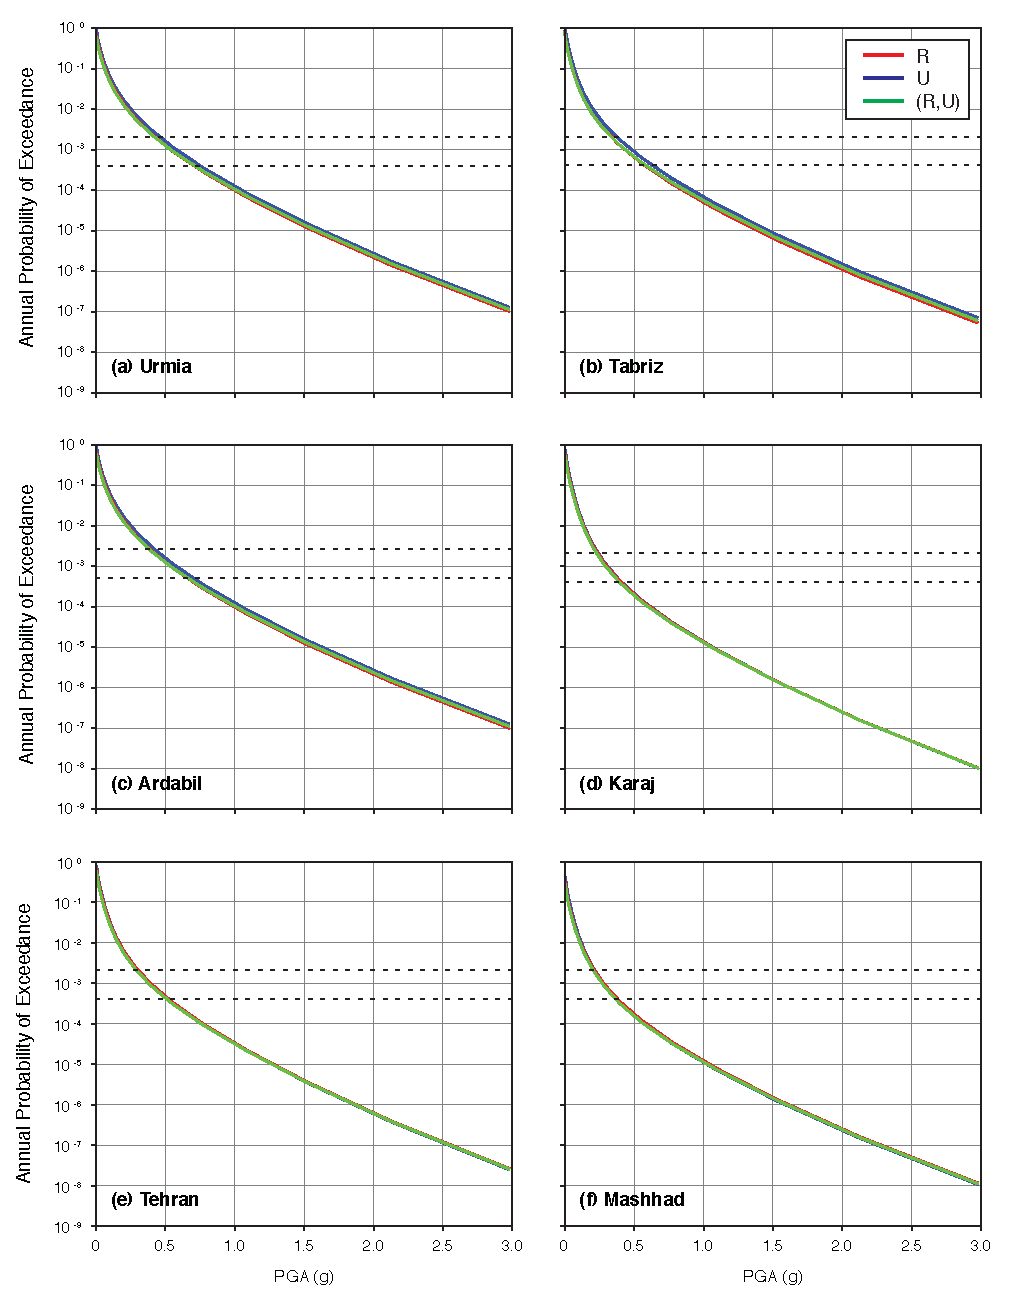
\includegraphics[width=\textwidth]{figures/pdf/figure-13}
    \caption{Hazard curves representing the annual probability of exceedance as function of peak ground acceleration for six cities in northern Iran based on the two basic models considered in this study, R and U, and the combined model (R,U). \myrevision{Dashed lines represent the 0.0021 and 0.000404 annual probability of exceedance corresponding to probability of exceedance of 10 and 2 percent in 50 years.}}
    \label{fig:hazardcurve}
\end{figure*}

\section{Results and Analysis}

Using the data, parameters, and procedures just described, we considered two different hazard models based on whether we use the five distinct seismic hazard regions or the whole area of interest as a uniform seismic hazard region. We call these the R and U models, respectively. Using these models we obtained hazard curves and expected PGA values for two probabilities of exceedance, at 2 and 10 percent in 50 years for events exceeding magnitudes \myrevision{$M_w \geq 4.5$}. These probabilities correspond to return periods of 475 and 2,475 years. For nomenclature purposes, we use the probabilities as a suffix on the model type. As an example, we refer to the results for 2 percent probability of exceedance in 50 years using the five-regions model as R2, whereas for the case of 10 percent probability of exceedance when using the uniform model we use the tag name U10.

Our choice for the threshold magnitude is based on the assumption that at the local scale (where a point of interest is close to the source), the hazard will be controlled by events \myrevision{$M_w \geq 4.5$}, or conversely, \myrevision{$M_{\min}$ was chosen based on the expected smallest magnitude capable of causing damage}. In turn, the 2 and 10 percent probability of exceedance in a \myrevision{50-year} span are considered a standard practice in seismic design, and are the probabilities used in the Iranian building code \citep{BHRC2014}.

In the R models, we computed the probability of exceedance of the ground motion separately for each region and then added their exceedance rates at a given level of ground motion in order to have the contribution of all regions for any given grid point within the region of interest. The results are obtained in the form of annual rate of exceedance. Expected PGA values are therefore a ``slice'' of the actual hazard curves cut across all grid points for a chosen exceedance rate.

Figure~\ref{fig:pga} shows the expected mean PGA values obtained for the R and U models, \myrevision{included the associated uncertainties in $b$, $M_{\max}$ and the GMPE. That is, the results in Fig.~\ref{fig:pga} correspond to the complete regional and uniform model branches in the logic tree for the different sub-models R2, R10, U2 and U10}. As can be expected, the highest PGA values are associated with the R2 and U2 models, and the lowest with the R10 and U10 models. For the R model results shown in Fig.~\ref{fig:pga}a, the highest levels of expected ground motion occur in the Azerbaijan region \myrevision{on the west side of the North Tabriz Fault and also on and around the border of the Kopeh Dagh and Alborz tectonic seismic regions on the east side of the North Alborz Fault. We also observe higher hazard in the Alborz region in a small area east from the Mosha Fault. On the other hand, the results shown in Fig.~\ref{fig:pga}b for the U model indicate that in addition to these areas, there are also large expected ground motions in the Zagros seismic zone and increased PGA results in various areas within the Central East seismic region}.

In general, the U models exhibit higher levels of expected ground motions when compared to their corresponding R models. This is illustrated in Fig.~\ref{fig:pga.diff}, which shows the difference between both models, U--R (U minus R). In this figure, positive values indicate that the U models have larger mean PGA values than the R models. \myrevision{As it can be seen, this is true practically throughout the whole region at very low levels, but more predominantly in the north-west region at a moderate level of up to 0.2 g and increasingly so in the Zagros region, where the differences between about 0.2 and 0.45 g. The higher results in the U model occurred because of higher $M_{max}$ and lower $b$ values in comparison with the R model}.

Overall, these results are consistent with the seismicity observed in Fig.~\ref{fig:catalog}. The R model results, however, seem to be more sensitive to the influence of large magnitude events observed in both the historical and modern seismicity maps, with a concentration of strong earthquakes in the Azerbaijan and Kopeh Dagh regios; whereas the U model results seem to be more sensitive to the influence of low-to-moderate magnitude events, especially in the Zagros and Central East regions.

\myrevision{With this in mind, and knowing that no one model (R or U) can be considered uniquely correct, we consider now the combination of both models as presented for the complete logic tree in Fig.~\ref{fig:logic}. We refer to this as the (R,U) model and the results are shown in Fig.~\ref{fig:pga.ru.std}, again in the form of expected mean PGA values for 2 and 10 percent in 50 years.}

\myrevision{The combined (R,U) model reflects the distribution of the region's seismicity shown in Fig.~\ref{fig:catalog} as well as that of the major faults shown in Fig.~\ref{fig:selected}a, but it also reflects the influence that small earthquakes have on the seismicity hazard of the region}. It displays well the contribution of the North Tabriz Fault system in the Azerbaijan region as well as the contribution of the North Alborz fault in the Alborz region and that of the different faults in the Kopeh Dagh region. In Fig.~\ref{fig:pga.ru.std}, the highest PGAs are observed in the (R,U)2 model results, where the expected accelerations are of the order of 1.0 g to the northwest of \myrevision{the} city of Tabriz. These maximum values should, nonetheless, be interpreted with caution given the fact that predictions are based on rock-site assumptions and do not include any kind of site effects or other related conditions which may often contribute to mitigating peak accelerations.

\myrevision{We also note that the overall distribution of mean PGA agrees with the recent study by \citet{Khodaverdian_2016_BSSA}. However, their results are in general slightly lower than ours. Obviously, given the differences in the catalogs, completeness magnitude, and in the seismicity parameters $M_{\max}$ and $b$, we cannot expect PGA values to match. For example, in the case of the $b$ values, \citet{Khodaverdian_2016_BSSA} reported large variations netween 0.56 and 1.27, where over 50 percent of the grid points had $b$ values greater than 1; whereas in our study the $b$ values observe a narrow range of variation between 0.93 and 1.15. In this regard we should note that \citet{Khodaverdian_2016_BSSA} computed the seismicity parameters for each grid point considering the contributions within a circular area of radius 200 m, whereas we considered a uniform seismicity parameters for each region and account for the uncertainty in the difference between regions via the combination of the R and U models.}

\myrevision{Altogether, on average, we found our results to be in good agreement with other previous results. For the city of Uremia, for instance, we obtained a expected PGA of 0.24 g, which is slightly lower than values obtained by \citet{BHRC2014} and \citet{Zare2012} and higher than \citet{Khodaverdian_2016_BSSA} for a 10 percent probability of exceedance in 50 years. We believe \citet{Zare2012} obtained higher values because their of use of a parametric method. For a 2 percent probability of exceedance in 50 years, \citet{Golara2014} obtained expected PGAs on the order of 0.3--0.5 g, where our mean value is 0.38 g. For the city of Tabriz, our results match with those obtained by \citet{BHRC2014} and are within the range of values computed by \citet{Zare2012}, for a 10 percent probability. These and other similar comparisons are summarized in Table \ref{tab:pga}, where we show our results and those of other previous studies for selected cities in northern Iran.}

\myrevision{As mentioned before, overall, our results are close to or within the ranges provided by most previous studies}. The only noticeable exceptions are the results of \citet{Golara2014}, whose expected PGA values are significantly higher than the rest. \myrevision{One possible explanation for the higher values in \citet{Golara2014} is their use of the maximum credible earthquake as the value for $M_{\max}$. The maximum credible earthquake is the largest earthquake that appears capable of occurring under the known tectonic framework for a specific fault or seismic source, based on geologic and seismic data. Therefore, it is often higher than historical documented observations or instrumental data-driven estimations of $M_{\max}$}.

Following the comparisons shown in Table \ref{tab:pga}, we looked into the more complete picture of the annual probabilities of exceedance as functions of PGA\myrevision{, also known as hazard curves. The results are shown in Fig.~\ref{fig:hazardcurve} for six of the main cities in northern Iran including the R, U, and the combined (R,U) models. Although for these particular cities, the differences are minor in general, they exemplify the results one can obtain at particular locations. Here, the more clear differences are observed for the city of Urmia, where the (R,U) model approaches the R model for low values of PGA and then evolves closer to the U model for higher values of PGA}.

\begin{figure}[t]
    \centering
    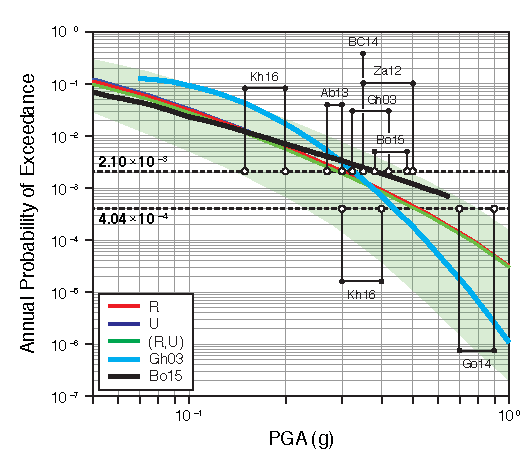
\includegraphics[width=0.48\textwidth]{figures/pdf/figure-14}
    \caption{Hazard curve comparison between the models considered in this study and the results of two previous studies by \citet{Ghodrati2003} and \citet{Boostan2015} for the city of Tehran. Here, the two previous studies just mentioned are identified with the codes Gh03 and Bo15, respectively. Also the PGA ranges of the \ref{tab:pga} are represented. The shaded area represents the upper and lower value of uncertainty at the GMPEs.}
    \label{fig:tehran}
\end{figure}

*** DONE UP TO HERE ***

\myrevision{Last, we concentrate our attention on the results for the capital city of Tehran. We compare hazard curves obtained in this study against those computed by \citet{Ghodrati2003} and \citet{Boostan2015} as well as ranges from other studies for 2 and 10\% probability of exceedance in 50 years. By applying different combination of magnitude (M) and distance (R), \citet{Boostan2015} presented a new model for probabilistic seismic hazard assessment based on fuzzy sets theory for Tehran, Iran. They expected to achieve higher seismic hazard values because of considering a vast uncertainty range for R and M. They concluded, non-fuzzy approaches due to not considering all uncertainties leads to non-conservative results. \citet{Ghodrati2003} conducted a probabilistic seismic hazard analysis for the same region based on considering the uncertainty in seismicity value and ground motion level through logic tree approach. They consider the uncertainty in seismicity parameters by involving the results of \citet{Tavakoli1999}. \citet{Tavakoli1999} reported the $b-value$ and $M_{max}$ as $0.52\pm0.02$ and $7.9\pm0.3$, respectively, which is fairly different from the result of this study. Even though   \citet{Ghodrati2003} used three GMPEs model,  \citet{Boostan2015} used only one model as attenuation relationship. As we discussed earlier, our model fairly well consider the ground motion level uncertainty.  Our results are similar to those obtained by \citet{Boostan2015} in the range between 0.1 and 0.3 g (corresponding to annual probabilities of exceedance between $10^{-3}$ and $10^{-1}$), and then it is in the mean range of the mentioned studies.  Conversely, the trend in the hazard curve from \citet{Boostan2015} suggest the city is to expect significantly higher levels of ground motion at higher probability rates, which is contrary to our findings and those of \citet{Ghodrati2003}. Expected PGA range of other studies mentioned at the \ref{tab:pga}, represents, on average, our study presents trustable results. The shaded area, represents the upper and lower value of uncertainty at the GMPEs. In other word the upper part edge is calculated by just considering GMPEs+Unc  and the lower edge is calculated by just considering GMPEs-Unc. It perfectly represents that almost all studies are in the range of uncertainty of the GMPEs, and using one appropriate backbone GMPE as well as the uncertainties could have better role in considering the epistemic uncertainty than using multiple GMPEs as \citet{Atkinson2014} concluded.}
